\documentclass{standalone}
\usepackage{tikz}
\usetikzlibrary{positioning, shapes.misc}

\begin{document}

\begin{tikzpicture}

% Placeholder image
\node[inner sep=0, outer sep=0] (image) at (0,0) {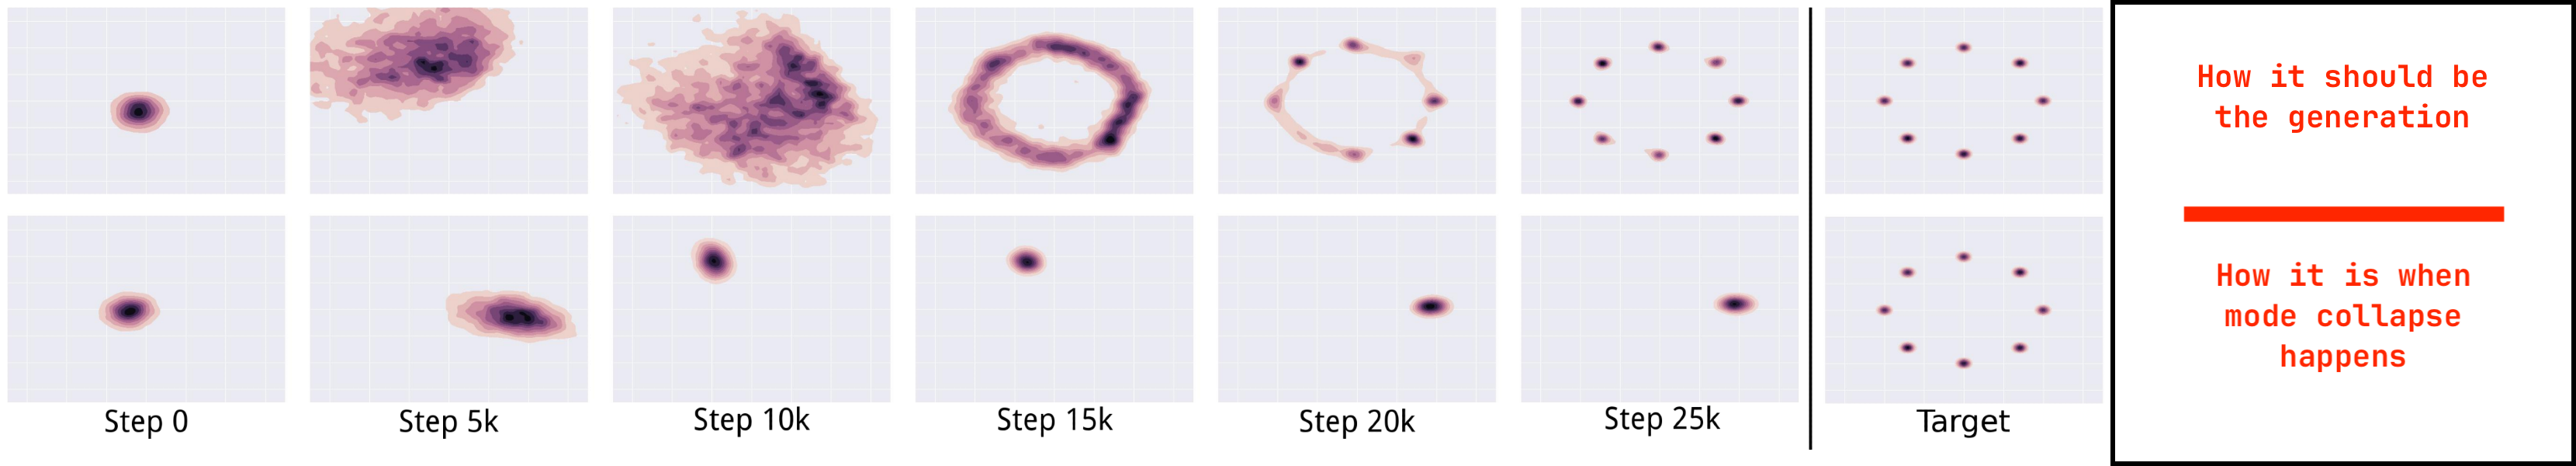
\includegraphics[width=24cm,height=6cm]{tikz/chapter9 - Mode Collapse HeatMap.png}};
\node[fill=white, xshift=0cm, yshift=-2.5cm, minimum width=24cm, minimum height=0.7cm] {};
\node[fill=white, xshift=-10.3cm, yshift=-2.58cm] {\large Step 0};
\node[fill=white, xshift=-6.9cm, yshift=-2.58cm] {\large Step 5K};
\node[fill=white, xshift=-3.4cm, yshift=-2.58cm] {\large Step 10K};
\node[fill=white, xshift=0cm, yshift=-2.58cm] {\large Step 15K};
\node[fill=white, xshift=3.4cm, yshift=-2.58cm] {\large Step 20K};
\node[fill=white, xshift=6.9cm, yshift=-2.58cm] {\large Step 25K};
\node[fill=white, xshift=10.3cm, yshift=-2.58cm] {\large Target};
\end{tikzpicture}

\end{document}